\documentclass[10pt,a4paper]{article}
\usepackage[utf8]{inputenc}
\usepackage[T1]{fontenc}
\usepackage{amsmath}
\usepackage{amssymb}
\usepackage{graphicx}
\usepackage{tikz}
\usetikzlibrary{bayesnet}
\author{Demetri Pananos}
\begin{document}
	
		\begin{figure}[t!]
		
		\centering
		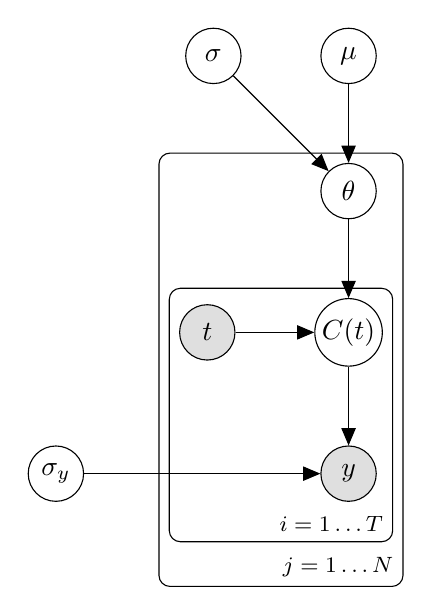
\begin{tikzpicture}
			
			\node[latent](mu){$\mu$};
			\node[latent, left=of mu](sig){$\sigma$};
			
			\node[latent, below = of mu](theta){$\theta$};
			
			
			\node[latent, below = of theta](C){$C(t)$};
			\node[obs, left = of C](t){$t$};
			\node[obs, below = of C](y){$y$};
			\node[latent, left = of y, xshift=-2cm](s){$\sigma_y$};
			\edge{sig}{theta};
			\edge{mu}{theta};
			\edge{theta}{C};
			\edge{t}{C};
			\edge{C}{y};
			\edge{s}{y};
			
			\plate[]{t_y_pairs}{(t)(y)(C)}{$i=1 \dots T$};
			\plate[]{subjects}{(t_y_pairs)(theta)}{$j=1 \dots N$};
			
		\end{tikzpicture}
		
	\end{figure}
	
	
	\begin{figure}[t!]
		
		\centering
		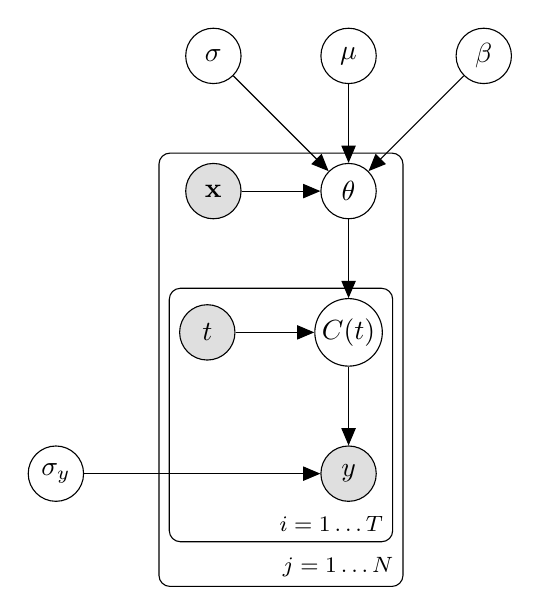
\begin{tikzpicture}
			
			\node[latent](mu){$\mu$};
			\node[latent, right=of mu](b){$\beta$};
			\node[latent, left=of mu](sig){$\sigma$};
			
			
			\node[latent, below = of mu](theta){$\theta$};
			\node[obs, left = of theta](x){$\mathbf{x}$};
			
			
			\node[latent, below = of theta](C){$C(t)$};
			\node[obs, left = of C](t){$t$};
			\node[obs, below = of C](y){$y$};
			\node[latent, left = of y, xshift=-2cm](s){$\sigma_y$};
			
			\edge{sig}{theta};
			\edge{b}{theta};
			\edge{mu}{theta};
			\edge{x}{theta};
			\edge{theta}{C};
			\edge{t}{C};
			\edge{C}{y};
			\edge{s}{y};
			
			\plate[]{t_y_pairs}{(t)(y)(C)}{$i=1 \dots T$};
			\plate[]{subjects}{(t_y_pairs)(x)(theta)}{$j=1 \dots N$};

		\end{tikzpicture}
		
	\end{figure}
	
	
	
	
	\begin{figure}[t!]
		
		\centering
		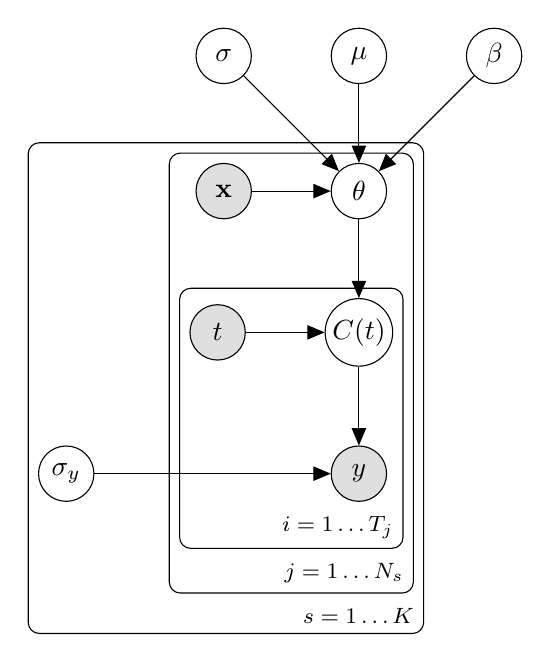
\begin{tikzpicture}
			
			\node[latent](mu){$\mu$};
			\node[latent, right=of mu](b){$\beta$};
			\node[latent, left=of mu](sig){$\sigma$};

			
			\node[latent, below = of mu](theta){$\theta$};
			\node[obs, left = of theta](x){$\mathbf{x}$};
			
			
			\node[latent, below = of theta](C){$C(t)$};
			\node[obs, left = of C](t){$t$};
			\node[obs, below = of C](y){$y$};
			\node[latent, left = of y, xshift=-2cm](s){$\sigma_y$};
			
			\edge{sig}{theta};
			\edge{b}{theta};
			\edge{mu}{theta};
			\edge{x}{theta};
			\edge{theta}{C};
			\edge{t}{C};
			\edge{C}{y};
			\edge{s}{y};
			
			\plate[]{t_y_pairs}{(t)(y)(C)}{$i=1 \dots T_j$};
			\plate[]{subjects}{(t_y_pairs)(x)(theta)}{$j=1 \dots N_s$};
			\plate[]{study}{(subjects)(s)}{$s=1 \dots K$};
		\end{tikzpicture}

	\end{figure}
	
	
	
	
\end{document}